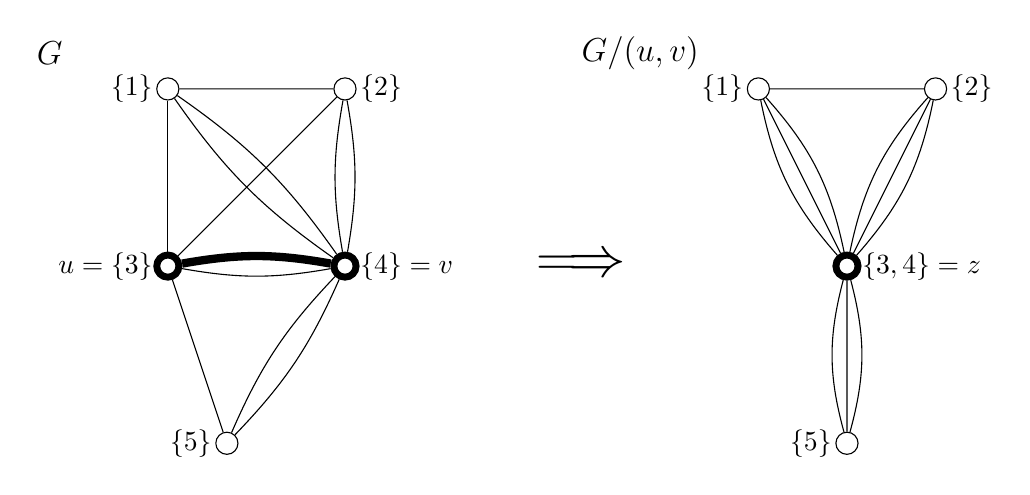
\begin{tikzpicture}[
    % Global styles
    vertex/.style={circle, draw=black, fill=white, inner sep=0pt, minimum size=8pt},
    boldvertex/.style={vertex, line width=2.5pt},
    scale=1.5  % Scaling up for better visibility
    ]
    % ===========================
    % LEFT GRAPH G
    % ===========================

    % Label G
    \node at (-1, 1.8) {\large $G$};

    % Nodes
    \node[vertex] (n1) at (0, 1.5) {};
    \node[vertex] (n2) at (1.5, 1.5) {};
    \node[boldvertex] (u) at (0, 0) {};
    \node[boldvertex] (v) at (1.5, 0) {};
    \node[vertex] (n5) at (0.5, -1.5) {};

    % Labels
    \node[left=2pt] at (n1) {$\{1\}$};
    \node[right=2pt] at (n2) {$\{2\}$};
    \node[left=2pt] at (u) {$u = \{3\}$};
    \node[right=2pt] at (v) {$\{4\} = v$};
    \node[left=2pt] at (n5) {$\{5\}$};

    % Edges
    % Top connections
    \draw (n1) -- (n2);
    \draw (n1) -- (u);
    \draw (n2) -- (u);
    \draw (n1) to[bend left=10] (v);
    \draw (n1) to[bend right=10] (v);

    % Multiple edges between 2 and v
    \draw (n2) to[bend right=10] (v);
    \draw (n2) to[bend left=10] (v);

    % Connection u-v (Thick line + 2 curves)
    \draw[line width=3pt] (u) to[bend left=10] (v);
    \draw (u) to[bend right=10] (v);

    % Bottom connections
    \draw (u) -- (n5);
    \draw (v) to[bend left=10] (n5);
    \draw (v) to[bend right=10] (n5);


    % ===========================
    % ARROW
    % ===========================
    \node at (3.5, 0) {\huge $\Longrightarrow$};


    % ===========================
    % RIGHT GRAPH G/(u,v)
    % ===========================

    % Shift coordinates by x=5
    \begin{scope}[shift={(5,0)}]

        % Label G/(u,v)
        \node at (-1, 1.8) {\large $G/(u, v)$};

        % Nodes
        \node[vertex] (rn1) at (0, 1.5) {};
        \node[vertex] (rn2) at (1.5, 1.5) {};
        % The contracted node z is roughly between where u and v were
        \node[boldvertex] (z) at (0.75, 0) {};
        \node[vertex] (rn5) at (0.75, -1.5) {};

        % Labels
        \node[left=2pt] at (rn1) {$\{1\}$};
        \node[right=2pt] at (rn2) {$\{2\}$};
        \node[right=2pt] at (z) {$\{3, 4\} = z$};
        \node[left=2pt] at (rn5) {$\{5\}$};

        % Edges
        % 1 to 2
        \draw (rn1) -- (rn2);

        % 1 to z
        \draw (rn1) to[bend left=15] (z);
        \draw (rn1) to[bend right=15] (z);
        \draw (rn1) -- (z);

        % 2 to z (3 edges)
        \draw (rn2) to (z);         % center
        \draw (rn2) to[bend left=15] (z);
        \draw (rn2) to[bend right=15] (z);

        % 5 to z (2 edges)
        \draw (rn5) to[bend left=15] (z);
        \draw (rn5) to[bend right=15] (z);
        \draw (rn5) -- (z);

    \end{scope}

\end{tikzpicture}